\documentclass{article}

\usepackage[utf8]{inputenc}
\usepackage[T1]{fontenc}
\usepackage{lipsum}
\usepackage{graphicx}
\usepackage{amsmath}
\usepackage[margin=1in]{geometry}
\usepackage{titlesec}
\usepackage{enumitem}

\titleformat{\section}
{\LARGE\bfseries}{\thesection}{1em}{}

\titleformat{\subsection}
{\Large\bfseries}{\thesection}{1em}{}

\begin{document}
\pagestyle{empty}
\section*{Design Pattern 3}
\large

\subsection*{Introduzione}
\large
Obiettivi:
\begin{itemize}
    \renewcommand{\labelitemi}{-}
    \itemsep0em
    \item Applicare propriamente i pattern del modello GoF 
\end{itemize}
Questa sezione rappresenta il naturale conseguimento del documento \textit{Design Pattern 2}, in cui sono elencati ulteriori pattern \textit{comportamentali}, \textit{creazionali} e \textit{strutturali} del \textit{catologo GoF}.

\subsection*{Singleton (Creational Pattern)}
\large 
\textit{Problema}\\
Come garantire che sia creata una sola istanza di una classe e fare in modo che sia condivisibile dagli elementi del modello?\vspace*{14pt}\\
\textit{Singleton} è un pattern creazionale adoperato per istanziare oggetti in maniera tale che siano rispettati i principi di qualità del software, cercando di manipolare al meglio le dipendenze tra le classi. La volontà di implementare un meccanismo simile, avviene qualora differenti elementi del dominio eseguano lo stesso processo esecutivo, da cui saranno restituiti certi \textit{behaviors} oppure dati in \textit{output}.\vspace*{14pt}\\
Per cui l'intento promuove la creazione di una singola istanza della classe software analizzata, affinchè essa possa essere condivisa tra le entità del sistema elaborato. Tendenzialmente è dichiarata come una variabile \textit{privata}, in quanto lo stesso \textit{costruttore} è \textit{protetto} oppure \textit{privato}, a cui si associa una funzione \textit{pubblica} che incapsula al suo interno l'intero codice di inizializzazione e provvede all'accesso all'instanza in questione.\vspace*{14pt}\\
\textit{Soluzione}\\
Creare una \textit{singola} istanza della classe software analizzata e provvedere ad un \textit{unico punto di accesso}.\vspace*{14pt}\\
Generalmente l'utilizzo di \textit{Singleton} avviene solo se soddisfatti tre criteri comportamentali, suddivisi in:
\begin{itemize}[label={-}]
    \itemsep0em
    \item Sviluppo progettuale secondo il principio \textit{lazy initialization}, ossia posticipare la creazione di un oggetto fino al momento in cui non sia realmente necessario 
    \item Non sia possibile attribuire ad alcun elemento del modello la \textit{responsabilità} della creazione dell'istanza
    \item Nonostante sia sviluppato un metodo pubblico per rendere accessibile l'oggetto della classe software, non deve essere garantita la possibilità che la funzione sia richiamabile a livello globale
\end{itemize}

\subsection*{Proxy (Structural Pattern)}
\large
\textit{Problema}\\
Come intercettare l'accesso di certi elementi del modello ad oggetti di ulteriori classi software?\vspace*{14pt}\\
In alcuni casi potrebbe essere desiderata la funzionalità che provveda ad accertarsi di quali istanze di classi software siano momentaneamente adoperate, oppure per controllare quali referenze, incapsulate all'interno dell'oggetto, siano attuate. Come già ribadito in capitoli precedenti, è possibile porre livelli di astrazione che operano come mediatori tra le entità del design project, caratterizzando la netta separazione tra \textit{high level classes} e \textit{low level classes} di un qualsiasi sistema software sviluppato. Riassumendo quanto detto è necessario introdurre un \textit{intermediario} tra il fornitore di funzionalità, legati alla business logic, e il richiedente, elemento affine all'utente finale.\vspace*{14pt}\\
\textit{Soluzione}\\
Realizzare un \textit{segnaposto} per controllare l'accesso agli oggetti interessati.\vspace*{14pt}\\
\textit{Caso di studio}\\
\begin{center}
    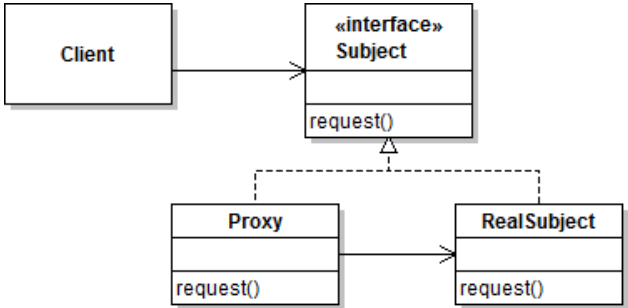
\includegraphics[width=0.5\textwidth]{foto 1.png}
\end{center}
La raffigurazione rispetta la soluzione del pattern \textit{Proxy}, in cui si visualizzano un totale di quattro entità. Nell'esempio proposto si contraddistinguono:
\begin{itemize}[label={-}]
    \itemsep0em
\item \textit{Client} è una \textit{high level class}, per cui affine all'impiego da parte di utenti finali
    \item \textit{Subject} indica il livello di astrazione richiesto per soddisfare il \textit{Dipendency Inversion Principle}, ossia l'isolamento di classi legate alla logica algoritmica rispetto a \textit{HLC}
    \item \textit{Proxy}, mediatore che prevede la concretizzazione della struttura \textit{request-response}, ossia rimane in attesa di ricevere \textit{richieste} affinchè possa restituire \textit{risposte inerenti}
    \item \textit{RealSubject} rappresenta la classe software soggetta a controlli pur di verificare il corretto utilizzo di istanze affiliate, caratterizzate dalle \textit{ } da oggetti esterni all'elemento del dominio
\end{itemize}
In questo contesto è la classe \textit{Proxy} che promuove lo smistamento di richieste e risposte, affinchè non siano violati i principi \textit{SOLID}, ovviando ad una scarsa qualità del codice, e attuando un meccanismo che possa soddisfare i requisiti imposti dalla classe cliente.\vspace*{14pt}\\
Concludendo, l'interfaccia potrebbe essere sostituita mediante una \textit{pure fabrication}, soddisfando il principio \textit{DIP}, grazie alla realizzazione di una specifica \textit{factory} implementata per la creazione di istanze, in questa tematica di tipologia \textit{Proxy}, le quali saranno conseguentemente restituite.

\subsection*{Intermezzo}
\large
Di seguito è illustrato un esempio che possa raffigurare certi contesti in cui il solo utilizzo di principi legati al paradigma degli oggetti non sia sufficiente per rispondere a caratteristiche comportamentali, oltre a diminuire la qualità del codice implementato.\vspace*{14pt}\\
\textit{Caso di studio}\\
\begin{center}
    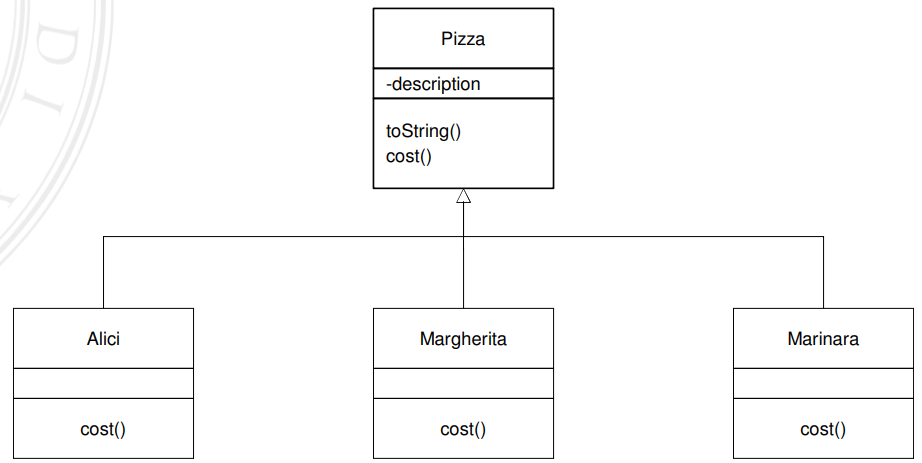
\includegraphics[width=0.7\textwidth]{foto 2.png}
\end{center}
Attuando una semplificazione dell'immagine proposta, affinchè un concetto simile possa essere adoperato per contesti generali, si sottolinea la presenza di una \textit{superclasse} e un totale di tre \textit{sottoclassi}, in cui è applicato il principio del \textit{poliformismo} in maniera tale che classi derivate possano adottare un'implementazione specifica dei \textit{metodi ereditati}.\\
Tuttavia, tale meccanismo di modellazione aumenta notevolmente la complessità architetturale, a causa del numero crescente di funzionalità che possano essere richieste, dove, in un domain model del genere, ogni \textit{classe figlia} richiede una propria specializzazione, formulando ricorsivamente condizioni di \textit{ereditarietà} e \textit{polimorfismo}.\vspace*{3pt}  
\begin{center}
    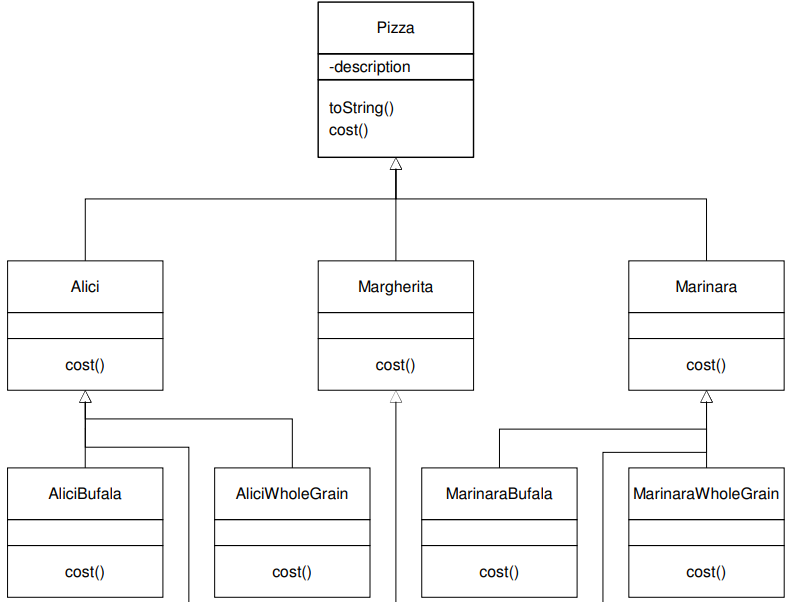
\includegraphics[width=0.7\textwidth]{foto 3.png}
\end{center}
Come già espresso in precedenza, ogni combinazione diviene una nuova entità da gestire, provocando un numero enorme di classi rappresentative all'interno del modello realizzato, in cui il metodo \textit{cost()}, incapsulato all'interno di sottoclassi finali, richiamerà la funzione per ogni termine antecedente, elaborando una consistente condizione di selezione (\textit{riferimento alla realizzazione di rami if-else annidati, contrari rispetto ad una software quality di spessore}).\vspace*{14pt}\\
Una risoluzione alternativa potrebbe consistere nell'inserimento delle \textit{combinazioni} citate all'interno della \textit{classe padre}, come attributi privati booleani, in cui il metodo \textit{cost()} incapsulato mantiene la spesa per ogni supplemento aggiunto; mentre ognuna delle \textit{classi derivate} ridefiniscono la funzione aggiungendo al prezzo il \textit{costo base}.\vspace*{7pt}
\begin{center}
    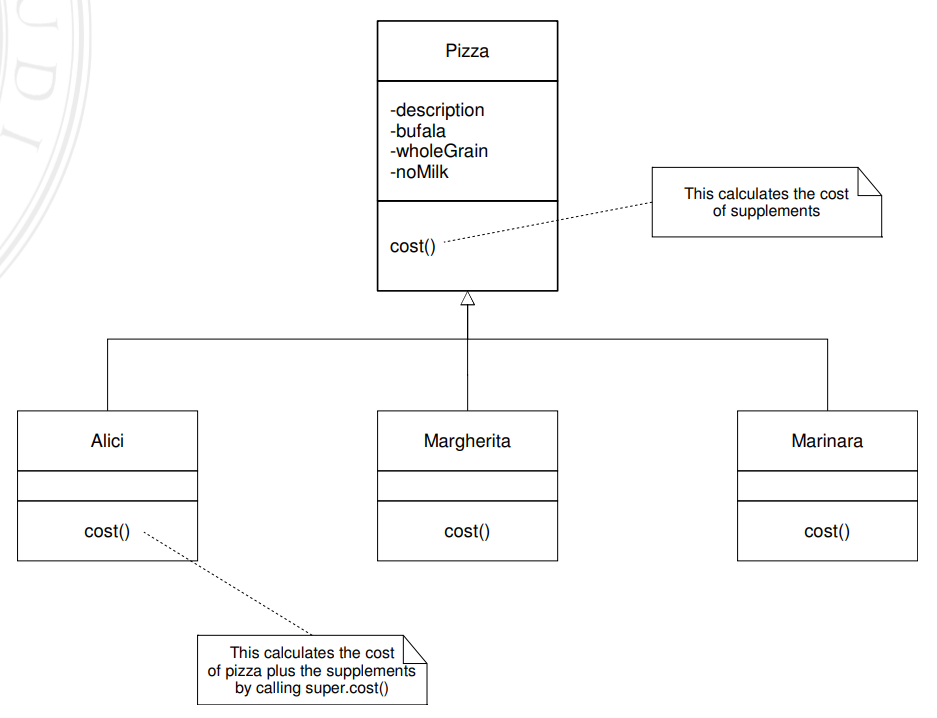
\includegraphics[width=0.7\textwidth]{foto 4.png}
\end{center}  
Nonostante raffiguri un approccio accettabile per implementare un sistema software con queste caratteristiche, è affetto da due problematiche, quali:
\begin{itemize}[label={-}]
    \itemsep0em
    \item Le \textit{classi derivate} durante il \textit{lifecycle} della soluzione sono soggette a modifiche, a cui si aggiungono le variazioni che i \textit{supplementi} possano subire; conseguentemente, ogni volta occorre correggere il metodo \textit{cost()}, a seconda dell'aggiunta oppure dell'eliminazione di nuove \textit{combinazioni}    
    \item \textit{Supplementi} sono modellati come un'unica entità, ma, come riportato nel \textit{domain model} di riferimento, nulla vieta che siano richieste \textit{combinazioni duplicate}, effettività che con attributi booleani non è permesso elaborare
\end{itemize} 

\subsection*{Decorator (Structural Pattern)}
\large
\textit{Problema}\\
Come potrebbero essere aggiunti comportamenti oppure stati ad istanze di classi software durante run-time?\vspace*{14pt}\\
L'intento consiste nell'aggiunta di \textit{behavior} ad oggetti individuali durante l'esecuzione del processo esecutivo, in quanto \textit{ineheritance} risulta essere \textit{statica} ed attuata all'intera classe software di riferimento, per cui non è flessibile a variazioni ricorrenti.\vspace*{7pt}\\
\textit{Decorator} tenta di rimediare alle mancanze precedenti, immettendo dinamicamente \textit{responsabilità} agli oggetti; inoltre, illustra un'alternativa molto più flessibile rispetto alla gerarchia composita di \textit{sottotipi}, la quale non si addice propriamente all'estensione di \textit{funzionalità}, e nemmeno alla creazione di nuovi metodi.\vspace*{7pt}\\
Rispetto al nuovo termine introdotto, affinchè sia appreso appieno il meccanismo del pattern in questione, è bene considerare \textit{Decorator} come se fosse un \textit{contenitore}. La soluzione include l'\textit{incapsulazione} dell'oggetto originario all'interno dell'entità \textit{decoratrici}, poichè i termini contraddistinti espongono della stessa interfaccia affinchè possano modellare lo stesso \textit{dominio}. Ai fini della descrizione attuata è proposta un'illustrazione grafica che possa chiarire quanto detto.
\begin{center}
    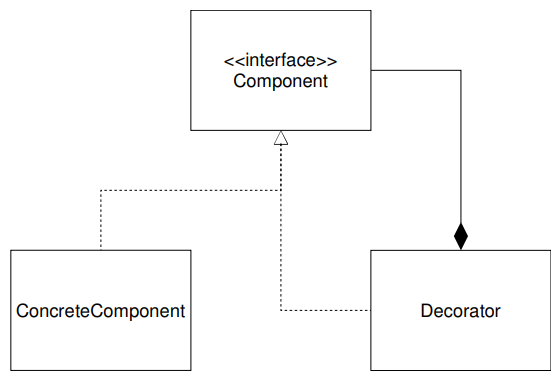
\includegraphics[width=0.4\textwidth]{foto 5.png}
\end{center} 
Si analizzano le componenti nella loro singolarità, in cui:
\begin{itemize}[label={-}]
    \itemsep0em
    \item \textit{ConcreteComponent}, entità software pertinente all'istanza di oggetti che possano essere successivamente arricchiti  
    \item \textit{Decorator}, classe decoratrice la quale rappresenta un certo comportamento o stato che possa essere aggiunto ad oggetti della classe concreta 
    \item \textit{Component}, interfaccia da cui i due termini precedenti ereditano attributi e metodi affini all'implementazione attuata
\end{itemize}
L'approccio prevede che i \textit{clienti}, ossia \textit{high level classes}, stabiliscano se vogliano aumentare la caratterizzazione comportamentale di oggetti relativi alla classe concreta, mediante l'utilizzo di decoratori; meccanismo reso possibile  dall'interfaccia \textit{Component}, in grado di soddisfare il \textit{Dipendency Inversion Priciple}, ma soprattutto sviluppando i \textit{comportamenti} affinchè siano legati alla stessa realtà modellativa, dato che ereditano attributi e metodi inerenti a \textit{ConcreteComponent}.

\subsection*{Adapter (Structural Pattern)}
\large
...
\end{document}